У даному розділі наведено опис аналітичного апарату, який використовується для розв'язання мішаних задач теорії пружності для прямокутної області.
Цей підхід базується на результати раніше проведених досліджень, зокрема робіт \cite{popov_1} і \cite{popov_2}.
Розглянута методика розв'язання мішаних плоских задач ґрунтується на застосуванні інтегральних перетворень безпосередньо до системи рівнянь рівноваги Ламе та крайових умов.
Це дозволяє зводити вихідну задачу до векторної одновимірної крайової задачі.
Векторна одновимірна крайова задача точно розв'язується за допомогою матричного диференційного числення та матричної функції Гріна.
Що призводить у результаті до сингулярного інтегрального рівнняння яке розв'язане за допомогою методу ортогональних многочленів описанного \cite{popov_3}.

\subsection{Постановка задачі}
\begin{figure}[h]
    \begin{center}
        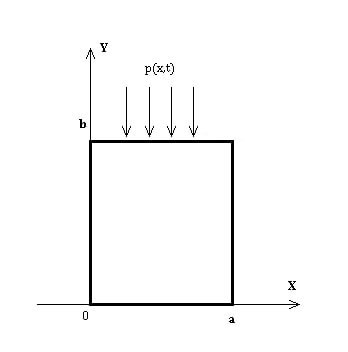
\includegraphics[scale=1]{images/geometry/image_4.jpg}
    \end{center}
    \caption{Геометрія проблеми}\label{geom_gen}
\end{figure}
Розглядається пружна прямокутна область (Рис: \ref{geom_gen}), яка займає область, що у декартовій системі координат описується співвідношенням $0 \le x \le a$, $0 \le y \le b$.

До прямокутної області на грані $y=b$ додане нормальне навантаження
\begin{equation}
    \sigma_y(x, y, t) |_{y=b} = -p(x, t), \quad  \tau_{xy}(x,y,t) |_{y=b} =0, \quad 0 \le x \le a
\end{equation}
де $p(x, t)$ відома функція.
На нижній грані виконуються наступні умови
\begin{equation}
    v(x,y,t) |_{y=0}, \quad \tau_{xy}(x,y,t) |_{y=0} =0
\end{equation}
На бічних гранях $x=0$ та $x=a$ граничні умови запишемо у формі
\begin{equation}\label{gen_bound_gen}
    U_1[f(x,y,t)]=0, \quad U_2[f(x,y,t)]=0 , \quad 0 \le y \le b
\end{equation}
Де 
\begin{align*}
    &U_1[f(x,y,t)]=\left[\alpha_1f(x,y,t) + \beta_1 \frac{\partial f(x,y,t)}{\partial x} \right]|_{x=0} \\
    &U_2[f(x,y,t)]=\left[\alpha_2f(x,y,t) + \beta_2 \frac{\partial f(x,y,t)}{\partial x} \right]|_{x=a} \\
\end{align*}
граничні функціонали у загальному виді (для кожної конкретної задачі вони будуть деталізовані), $f(x,y,t)=(u(x,y,t), v(x,y,t))^T$ - вектор переміщеннь.

Розглядаються наступні рівняння рівноваги Ламе:
\begin{equation}
    \begin{cases}
        \frac{\partial^2 u(x,y,t)}{\partial x^2} + \frac{\partial^2 u(x,y,t)}{\partial y^2} + \mu_0 (\frac{\partial^2 u(x,y,t)}{\partial x^2} + \frac{\partial^2 v(x,y,t)}{\partial x\partial y}) = \frac{1}{c_1^2} \frac{\partial^2 u(x,y,t)}{\partial t^2} \\
        \frac{\partial^2 v(x,y,t)}{\partial x^2} + \frac{\partial^2 v(x,y,t)}{\partial y^2} + \mu_0 (\frac{\partial^2 u(x,y,t)}{\partial x \partial y} + \frac{\partial^2 v(x,y,t)}{\partial y^2}) = \frac{1}{c_2^2} \frac{\partial^2 v(x,y,t)}{\partial t^2} \\
    \end{cases}
\end{equation}

Будемо розглядати випадок гармонічних коливань, тому можемо предствавити функції у наступному вигляді:
\begin{equation}
    u(x,y,t) = u(x,y) e^{i \omega t}, \quad v(x,y,t) = v(x,y) e^{i \omega t}, \quad p(x,t) = p(x) e^{i \omega t}
\end{equation}
Таким чином отримаємо наступні рівняння рівноваги:
\begin{equation}\label{lame_gen}
    \begin{cases}
        \frac{\partial^2 u(x,y)}{\partial x^2} + \frac{\partial^2 u(x,y)}{\partial y^2} + \mu_0 (\frac{\partial^2 u(x,y)}{\partial x^2} + \frac{\partial^2 v(x,y)}{\partial x\partial y}) = -\frac{\omega^2}{c_1^2}  u(x,y) \\
        \frac{\partial^2 v(x,y)}{\partial x^2} + \frac{\partial^2 v(x,y)}{\partial y^2} + \mu_0 (\frac{\partial^2 u(x,y)}{\partial x \partial y} + \frac{\partial^2 v(x,y)}{\partial y^2}) = -\frac{\omega^2}{c_2^2} v(x,y) \\
    \end{cases}
\end{equation}
Та граничні умови:
\begin{equation}\label{bound_gen}
    \begin{cases}
        \sigma_y(x, y) |_{y=b} = -p(x), \quad  \tau_{xy}(x,y) |_{y=b} =0 \\
        v(x,y) |_{y=0}, \quad \tau_{xy}(x,y) |_{y=0} =0 \\
        U_1[f(x,y)]=0, \quad U_2[f(x,y)]=0
    \end{cases}
\end{equation}

Введемо невідомі функції $\chi_1(y) = u(0, y)$, $\chi_2(y) = v(0, y)$, $\chi_3(y) = u(a, y)$, $\chi_4(y) = v(a, y)$.
Враховучи умову \eqref{gen_bound_gen}, отримаємо, що 
$\frac{\partial u(0, y)}{\partial x}=-\frac{\alpha_1}{\beta_1} \chi_1(y)$,
$\frac{\partial v(0, y)}{\partial x}=-\frac{\alpha_1}{\beta_1} \chi_2(y)$,
$\frac{\partial u(a, y)}{\partial x}=-\frac{\alpha_2}{\beta_2} \chi_3(y)$,
$\frac{\partial v(a, y)}{\partial x}=-\frac{\alpha_2}{\beta_2} \chi_4(y)$.
Отже умова \eqref{gen_bound_gen} виконується автоматично.

\subsection{Зведення задачі до одновимірної у просторі трансформант та її розв'язання}
Для того, щоб звести задачу до одновимірної задачі, використаємо інтегральне перетворення Фур'є по змінній $x$ до рівнянь \eqref{lame_gen} в наступному вигляді:
\begin{equation}
    \begin{pmatrix}
        u_n(y) \\
        v_n(y)
    \end{pmatrix} = \int_{0}^{a} 
    \begin{pmatrix}
        u(x,y) sin(\alpha_n x) \\
        v(x,y) cos(\alpha_n x)
    \end{pmatrix} dx, \quad \alpha_n = \frac{\pi n}{a}
\end{equation}

Для цього помножимо перше та друге рівняння \eqref{lame_gen} на $sin(\alpha_n x)$ та $cos(\alpha_n x)$ відповідно та проінтегруємо по змінній $x$ на інтервалі $0 \le x \le a$.
Покрокове інтегрування рівняння \eqref{lame_gen} наведено у (\nameref{ap_A}).
Отримана система рівнянь задачі у просторі трансформант:
\begin{equation}\label{transf_gen}
    \begin{cases}
        u_n^{''}(y) - \alpha_n \mu_0 v_n^{'}(y) - (\alpha_n^2 + \alpha_n^2 \mu_0 - \frac{\omega^2}{c_1^2}) u_n(y) = \\
        = \alpha_n(1 + \mu_0)(\chi_3(y) cos(\alpha_n a) - \chi_1(y)) \\
        \\
        (1 + \mu_0) v_n^{''}(y) + \alpha_n \mu_0 u_n^{'}(y) - (\alpha_n^2 - \frac{\omega^2}{c_2^2}) v_n(y) = \\
        = (\frac{\alpha_2}{\beta_2}\chi_4(y) cos(\alpha_n a) - \frac{\alpha_1}{\beta_1}\chi_2(y)) - \mu_0 (\chi_3^{'}(y) cos(\alpha_n a) -\chi_1^{'}(y))
    \end{cases}
\end{equation}

Застосовуючи інтегральне перетворення до граничних умов,
отримаємо наступні умови задачі у просторі трансформант:
\begin{equation}\label{transf_bound_gen}
    \begin{cases}
        \left( (2G + \lambda)v_n^{'}(y) + \alpha_n \lambda u_n(y) \right)|_{y=b} = -p_n \\
        \left(u_n^{'}(y) - \alpha_n v_n(y)  \right)|_{y=b} = 0 \\
        v_n(y)|_{y=0} = 0 \\
        \left(u_n^{'}(y) - \alpha_n v_n(y)  \right)|_{y=0} = 0
    \end{cases}
\end{equation}
де $p_n = \int_{0}^{a} p(x) cos(\alpha_n x) dx$

% \subsection{Зведення задачі у просторі трансформант до матрично-векторної форми}
Для того щоб розв'язати задачу у простосторі трансформант, перепишмо її у матрично-векторній формі.
Рівняння рівноваги \eqref{transf_gen} запишемо у наступному вигляді:
\begin{align}\label{transf_mat_gen}
    &L_2\left[ Z_n(y) \right] = A * Z_n^{''}(y) + B * Z_n^{'}(y) + C * Z_n(y) \nonumber \\
    &L_2\left[ Z_n(y) \right] = F_n(y)
\end{align}
Де
\begin{equation*}
    A = \begin{pmatrix}
        1 & 0 \\
        0 & 1 + \mu_0
    \end{pmatrix}, \quad
    B = \begin{pmatrix}
        0 & -\alpha_n \mu_0 \\
        \alpha_n \mu_0 & 0
    \end{pmatrix}
\end{equation*}
\begin{equation*}
    C = \begin{pmatrix}
        -\alpha_n^2 -\alpha_n^2 \mu_0 + \frac{\omega^2}{c_1^2} & 0 \\
        0 & -\alpha_n^2 + \frac{\omega^2}{c_2^2}
    \end{pmatrix}, \quad
    Z_n(y) = \begin{pmatrix}
        u_n(y) \\
        v_n(y)
    \end{pmatrix}
\end{equation*}
\begin{equation*}
    F_n(y) = \begin{pmatrix}
        \alpha_n(1 + \mu_0)(\chi_3(y) cos(\alpha_n a) - \chi_1(y)) \\
        (\frac{\alpha_2}{\beta_2}\chi_4(y) cos(\alpha_n a) - \frac{\alpha_1}{\beta_1}\chi_2(y)) - \mu_0 (\chi_3^{'}(y) cos(\alpha_n a) -\chi_1^{'}(y))
    \end{pmatrix}
\end{equation*}
Граничні умови \eqref{transf_bound_gen} запишемо у наступному вигляді:
\begin{align}\label{transf_bound_mat_gen}
    &U_i\left[ Z_n(y) \right] = E_i * Z_n^{'}(b_i) + F_i * Z_n(b_i) \nonumber \\
    &U_i\left[ Z_n(y) \right] = D_i
\end{align}
де $i = \overline{0, 1}$, $b_0 = b$, $b_1 = 0$,
\begin{equation*}
    E_0 = \begin{pmatrix}
        1 & 0 \\
        0 & 2G + \lambda
    \end{pmatrix}, \quad
    F_0 = \begin{pmatrix}
        0 & -\alpha_n \\
        \alpha_n \lambda & 0
    \end{pmatrix}, \quad
\end{equation*}
\begin{equation*}
    E_1 = \begin{pmatrix}
        1 & 0 \\
        0 & 0
    \end{pmatrix}, \quad
    F_1 = \begin{pmatrix}
        0 & -\alpha_n \\
        0 & 1
    \end{pmatrix}, \quad
\end{equation*}
\begin{equation*}
    D_0 = \begin{pmatrix}
        0 \\
        -p_n
    \end{pmatrix}, \quad
    D_1 = \begin{pmatrix}
        0 \\
        0
    \end{pmatrix}, \quad
\end{equation*}

Для знаходження розв'язку задачі у просторі трансформант, знайдем фундаментальну матрицю рівняння \eqref{transf_mat_gen}.
Шукати її будем у наступному вигляді \cite{gantmaher}:
\begin{equation}
    Y(y) = \frac{1}{2\pi i} \oint_C e^{sy} M^{-1}(s)ds
\end{equation}
де $M(s)$ - характерестична матриця рівняння \eqref{transf_mat_gen}, а $C$ - замкнений контур який містить усі особливі точки $M^{-1}(s)$. $M(s)$ будемо шукати з наступної умовни
\begin{equation}
    L_2\left[ e^{sy}*I \right] = e^{sy} * M(s), \quad I = \begin{pmatrix} 1 & 0 \\ 0 & 1 \end{pmatrix}
\end{equation}
\begin{align*}
    &L_2\left[ e^{sy}*I \right] = e^{sy} \left( s^2A * I + s B*I + C*I \right) = \\
    &=e^{sy} \begin{pmatrix}
        s^2 - \alpha_n^2 - \alpha_n^2\mu_0 + \frac{\omega^2}{c_1^2} & -\alpha_n \mu_0 s \\
        \alpha_n \mu_0 s & s^2 (1 + \mu_0) -\alpha_n^2 + \frac{\omega^2}{c_1^2}
     \end{pmatrix} \Rightarrow
\end{align*}

\begin{equation}
    M(s) = \begin{pmatrix}
        s^2 - \alpha_n^2 - \alpha_n^2\mu_0 + \frac{\omega^2}{c_1^2} & -\alpha_n \mu_0 s \\
        \alpha_n \mu_0 s & s^2 (1 + \mu_0) -\alpha_n^2 + \frac{\omega^2}{c_2^2}
     \end{pmatrix}
\end{equation}

Знайдемо тепер $M^{-1}(s) = \frac{\widetilde{M(s)}}{det[M(s)]}$.
\begin{equation}
    \widetilde{M(s)} = \begin{pmatrix}
        s^2 (1 + \mu_0) -\alpha_n^2 + \frac{\omega^2}{c_2^2} & \alpha_n \mu_0 s \\
        -\alpha_n \mu_0 s & s^2 - \alpha_n^2 - \alpha_n^2\mu_0 + \frac{\omega^2}{c_1^2}
     \end{pmatrix}
\end{equation}
\begin{align}
    &det[M(s)] = \begin{vmatrix}
        s^2 - \alpha_n^2 - \alpha_n^2\mu_0 + \frac{\omega^2}{c_1^2} & -\alpha_n \mu_0 s \\
        \alpha_n \mu_0 s & s^2 (1 + \mu_0) -\alpha_n^2 + \frac{\omega^2}{c_2^2}
     \end{vmatrix} = \nonumber \\
    &=(s - s_1)(s + s_1)(s - s_2)(s + s_2)
\end{align}
де $s_1$, $s_2$, $-s_1$, $-s_2$ корені $det[M(s)]=0$, детальне знаходження яких наведено в (\nameref{ap_B}).

Враховучи це, знайдемо значення фундаментальної матрицю за допомогою теореми про лишки:
\begin{align*}
    &\frac{1}{2\pi i} \oint_C e^{sy} M^{-1}(s)ds = \frac{2 \pi i}{2 \pi i (1 + \mu_0)} \sum_{i=1}^{4} Res\left[ e^{sy} \frac{\widetilde{M(s)}}{det[M(s)]} \right] = \\
    & = \left(Y_0(y) + Y_1(y) + Y_2(y) + Y_3(y) \right)
\end{align*}
Знайдемо $Y_0(y)$:
\begin{align}
    &Y_0(y) =  \left( \frac{e^{sy}}{(s+s_1)(s - s_2)(s + s_2)} \widetilde{M(s)} \right) \Big|_{s=s_1} = \nonumber \\
    &=\frac{e^{s_1 y}}{2s_1 (s_1^2 - s_2^2)} \begin{pmatrix}
        s_1^2 (1 + \mu_0) -\alpha_n^2 + \frac{\omega^2}{c_2^2} & \alpha_n \mu_0 s_1 \\
        -\alpha_n \mu_0 s_1 & s_1^2 - \alpha_n^2 - \alpha_n^2\mu_0 + \frac{\omega^2}{c_1^2}
    \end{pmatrix}
\end{align}
Знайдемо $Y_1(y)$:
\begin{align}
    &Y_1(y) =  \left( \frac{e^{sy}}{(s-s_1)(s - s_2)(s + s_2)} \widetilde{M(s)} \right) \Big|_{s=-s_1} = \nonumber \\
    &=-\frac{e^{-s_1 y}}{2s_1 (s_1^2 - s_2^2)} \begin{pmatrix}
        s_1^2 (1 + \mu_0) -\alpha_n^2 + \frac{\omega^2}{c_2^2} & -\alpha_n \mu_0 s_1 \\
        \alpha_n \mu_0 s_1 & s_1^2 - \alpha_n^2 - \alpha_n^2\mu_0 + \frac{\omega^2}{c_1^2}
    \end{pmatrix}
\end{align}
Знайдемо $Y_2(y)$:
\begin{align}
    &Y_2(y) =  \left( \frac{e^{sy}}{(s+s_2)(s - s_1)(s + s_1)} \widetilde{M(s)} \right) \Big|_{s=s_2} = \nonumber \\
    &=\frac{e^{s_2 y}}{2s_2 (s_2^2 - s_1^2)} \begin{pmatrix}
        s_2^2 (1 + \mu_0) -\alpha_n^2 + \frac{\omega^2}{c_2^2} & \alpha_n \mu_0 s_2 \\
        -\alpha_n \mu_0 s_2 & s_2^2 - \alpha_n^2 - \alpha_n^2\mu_0 + \frac{\omega^2}{c_1^2}
    \end{pmatrix}
\end{align}
Знайдемо $Y_3(y)$:
\begin{align}
    &Y_3(y) =  \left( \frac{e^{sy}}{(s-s_2)(s - s_1)(s + s_1)} \widetilde{M(s)} \right) \Big|_{s=-s_2} = \nonumber \\
    &=-\frac{e^{-s_2 y}}{2s_2 (s_2^2 - s_1^2)} \begin{pmatrix}
        s_2^2 (1 + \mu_0) -\alpha_n^2 + \frac{\omega^2}{c_2^2} & -\alpha_n \mu_0 s_2 \\
        \alpha_n \mu_0 s_2 & s_2^2 - \alpha_n^2 - \alpha_n^2\mu_0 + \frac{\omega^2}{c_1^2}
    \end{pmatrix}
\end{align}

\subsection{Побудова матриці-функції Гріна}
Для побудови матриці-функції Гріна спочатку знайдемо тепер фундамельні бизисні матриці $\Psi_0(y)$, $\Psi_1(y)$, шукати їх будем у наступному вигляді:
\begin{equation}\label{psi_gen}
    \Psi_i(y) = \left( Y_0(y) + Y_1(y) \right) * C_1^i + \left( Y_2(y) + Y_3(y) \right) * C_2^i
\end{equation}

Залишилось знайти невідомі матриці коєфіцієнтів $C_1^0$, $C_2^0$, $C_1^1$, $C_2^1$ використовуючи граничні умови \eqref{transf_bound_mat_gen}.
Покрокове знаходження яких наведено у (\nameref{ap_C}).
Для подальшого введемо наступні позначення для елементів матриць $\Psi_0(y)$, $\Psi_1(y)$:
\begin{equation*}
    \Psi_0(y) = \begin{pmatrix}
        \Psi_1^0(y) &  \Psi_2^0(y) \\
        \Psi_3^0(y) &  \Psi_4^0(y) 
    \end{pmatrix}, \quad 
    \Psi_1(y) = \begin{pmatrix}
        \Psi_1^1(y) &  \Psi_2^1(y) \\
        \Psi_3^1(y) &  \Psi_4^1(y) 
    \end{pmatrix}      
\end{equation*}

Таким чином матрицю Гріна можемо записати у вигляді:
\begin{equation}
    G(y,\xi) = 
    \begin{cases}
        \Psi_0(y) * \Psi_1(\xi), \quad 0 \le y < \xi \\
        \Psi_1(y) * \Psi_0(\xi), \quad \xi < y \le b
    \end{cases}
\end{equation}

Для данної матриці Гріна виконано усі властивості, зокрема виконані однорідні граничні умови \eqref{transf_bound_mat_gen}
та однорідні рівняння рівноваги у просторі трансформант \eqref{transf_mat_gen}:
\begin{equation*}
    L_2\left[  G(y, \xi) \right] = 0
\end{equation*}
\begin{equation*}
    U_0\left[ G(y, \xi) \right] = 0, \quad  U_1\left[ G(y, \xi) \right] = 0,
\end{equation*}

Таким чином ми можемо записати розв'язок крайової задачі у просторі трансформант:
\begin{equation}
    Z_n(y) = \int_0^b G(y,\xi) F_n(\xi) d\xi + \Psi_0(y) * D_0 + \Psi_1(y) * D_1
\end{equation}

Введемо наступні позначення $G(y, \xi) = \begin{pmatrix}
    g_1(y,\xi) & g_2(y,\xi) \\
    g_3(y,\xi) & g_4(y,\xi)
\end{pmatrix}$, $F_n(y) = \begin{pmatrix}
    f_n^1(y) \\
    f_n^2(y)
\end{pmatrix}$. Враховуючи це, шукані функціі перемішень у просторі трансформант можна записати у наступному вигляді
\begin{align}\label{transf_sol_u_gen}
    &u_n(y) = \int_0^b \left[g_1(y, \xi)f_n^1(\xi) + g_2(y, \xi)f_n^2(\xi) \right]d\xi - \psi_0^2(y) p_n
\end{align}
\begin{align}\label{transf_sol_v_gen}
    &v_n(y) = \int_0^b \left[g_3(y, \xi)f_n^1(\xi) + g_4(y, \xi)f_n^2(\xi) \right]d\xi - \psi_0^4(y) p_n
\end{align}

% \subsection{Побудова розв'язоку вихідної задачі}
Викорустовуючи обернене інтегральне перетворення Фур'є до розв'язку задачі у просторі трансформант
(\ref{transf_sol_u_gen}), (\ref{transf_sol_v_gen}), отримаємо фінальний розв'язок задачі
\begin{equation}
    u(x,y) = \frac{2}{a} \sum_{n=1}^{\infty} u_n(y) sin(\alpha_n x), \quad \alpha_n = \frac{\pi n}{a}
\end{equation}
\begin{equation}
    v(x,y) = \frac{v_0(y)}{a} + \frac{2}{a} \sum_{n=1}^{\infty} v_n(y) cos(\alpha_n x), \quad \alpha_n = \frac{\pi n}{a}
\end{equation}

Знайдем тепер $v_0(y)$ розглянувши задачу у просторі трансформант \eqref{transf_gen}, \eqref{transf_bound_gen} при $n=0$, $\alpha_n = 0$.
Детальний розв'язок якої наведено в (\nameref{ap_D}). Тоді остаточний розв'язок $v(x,y)$ буде мати вигляд
\begin{align}
    &v(x,y) = \frac{2}{a} \sum_{n=1}^{\infty} v_n(y) cos(\alpha_n x) - \psi_0(y) \frac{p_0}{a(2G + \lambda)} + \nonumber \\
    &+ \frac{1}{a(1+\mu_0)} \int_{0}^{b}g(y,\xi) [ (\frac{\alpha_2}{\beta_2}\chi_4(\xi) cos(\alpha_n a) - \frac{\alpha_1}{\beta_1}\chi_2(\xi)) - \nonumber \\
    & - \frac{\mu_0}{(1+\mu_0)} (\chi_3^{'}(\xi) cos(\alpha_n a) -\chi_1^{'}(\xi)) ] d\xi
\end{align}

Залишилось знайти невідомі функції $\chi_1(y)$, $\chi_2(y)$, $\chi_3(y)$, $\chi_4(y)$.
В подальшому в данній роботі розглянуто випадок таких граничних умов які призводять лише до однієї невідомої функції $f(y) = \frac{\partial v(x,y)}{\partial x}|_{x=a}$.
Для знаходження якої буде побудовано інтегральне рівняння завдяки граничній умові $\sigma_y(x, y) |_{y=b} = -p(x)$.

\subsection{Загальна схема розв'язку сінгулярного інтегрального рівняння}
Розглянемо випадок граничних умов другої основної задачі теорії пружності, в результаті отримаємо лише одну невідому функцію $f(y) = \frac{\partial v(x,y)}{\partial x}|_{x=a}$.
З цього отримаємо значення $f_n^1(\xi) = 0$, $f_n^2(\xi)= -cos(\alpha_n a) f(\xi)$.
Запишемо тепер фінальний розв'язок для цього випадку:
\begin{equation}
    u(x,y) = -\frac{2}{a} \sum_{n=1}^{\infty} \left( \int_0^b \left[g_2(y, \xi)cos(\alpha_n a) f(\xi) \right]d\xi + \psi_0^2(y) p_n \right) sin(\alpha_n x)
\end{equation}
\begin{align}
    &v(x,y) = -\frac{1}{a(1+\mu_0)} \int_{0}^{b}g(y,\xi) f(\xi) d\xi - \psi_0(y) \frac{p_0}{a(2G + \lambda)} \nonumber \\
    &- \frac{2}{a} \sum_{n=1}^{\infty} \left( \int_0^b \left[g_4(y, \xi) cos(\alpha_n a) f(\xi) \right]d\xi + \psi_0^4(y) p_n  \right) cos(\alpha_n x)
\end{align}

Використиємо граничну умову $\sigma_y(x, y) |_{y=b} = -p(x)$ для того, щоб отримати інтегральне рівняння:
\begin{equation*}
    (2G + \lambda)\frac{\partial v(x,y)}{\partial y}|_{y=b} + \lambda\frac{\partial u(x,y)}{\partial x}|_{y=b} = -p(x) \Leftrightarrow
\end{equation*}
\begin{align*}
    &-\frac{(2G + \lambda)}{a(1+\mu_0)} \int_{0}^{b}\frac{\partial g(y, \xi)}{\partial y}|_{y=b} f(\xi) d\xi - \psi_0^{'}(b) \frac{p_0}{a} - \\
    &- \frac{2(2G + \lambda)}{a} \frac{\partial}{\partial y} \sum_{n=1}^{\infty} \left( \int_0^b \left[g_4(y, \xi) cos(\alpha_n a) f(\xi) \right]d\xi + \psi_0^{4}(y) p_n \right) \\ 
    &cos(\alpha_n x)|_{y=b} - \frac{2\lambda}{a} \frac{\partial}{\partial x} \sum_{n=1}^{\infty} \left( \int_0^b \left[g_2(y, \xi)cos(\alpha_n a) f(\xi) \right]d\xi + \psi_0^2(y) p_n \right) \\ 
    &sin(\alpha_n x)|_{y=b} = -p(x)
\end{align*}
Введемо позначення:
\begin{align}
    &a_1(x) = a p(x) - 2(2G + \lambda) \frac{\partial}{\partial y} \sum_{n=1}^{\infty} \psi_0^{4}(y) p_n cos(\alpha_n x)|_{y=b} - \nonumber \\
    &- 2\lambda \frac{\partial}{\partial x} \sum_{n=1}^{\infty}\psi_0^2(y) p_n sin(\alpha_n x)|_{y=b} - \psi_0^{'}(b) p_0
\end{align}
Враховуючи його отримаємо наступне інтегральне рівняння відносно $f(\xi)$:
\begin{align}\label{int_gen}
    &\frac{(2G + \lambda)}{(1+\mu_0)} \int_{0}^{b}\frac{\partial g(y, \xi)}{\partial y}|_{y=b} f(\xi) d\xi + \nonumber \\ 
    &+ \int_{0}^{b} \sum_{n=1}^{\infty} cos(\alpha_n a) cos(\alpha_n x) \left[(2G + \lambda) \frac{\partial g_4(y, \xi)}{\partial y} + \alpha_n \lambda g_2(y, \xi) \right]|_{y=b} \nonumber \\
    &f(\xi) d\xi = a_1(x)
\end{align}
Розглянемо ряд:
\begin{align*}
    &\sum_{n=1}^{\infty} cos(\alpha_n a) cos(\alpha_n x) \left[(2G + \lambda) \frac{\partial g_4(y, \xi)}{\partial y} + \alpha_n \lambda g_2(y, \xi) \right]|_{y=b} = \\
    &= \sum_{n=1}^{\infty} (-1)^n \alpha_n^{-1} e^{\alpha_n (\xi - b)} cos(\alpha_n x) \left[ \frac{\partial \widetilde{g_4(y, \xi)}}{\partial y} + \lambda \widetilde{g_2(y, \xi)} \right]|_{y=b} = \\
    &= \sum_{n=1}^{N} (-1)^n \alpha_n^{-1} e^{\alpha_n (\xi - b)} cos(\alpha_n x) \left[ \frac{\partial \widetilde{g_4(y, \xi)}}{\partial y} + \lambda \widetilde{g_2(y, \xi)} \right]|_{y=b} + \\
    & + a_2 \sum_{n=N}^{\infty} (-1)^n (2n + 1)^{-1} e^{-(2n + 1) \frac{\pi}{2a} (b - \xi)} cos((2n + 1) \frac{\pi}{2a} x) + \\
    & + a_2 \sum_{n=0}^{N} (-1)^n (2n + 1)^{-1} e^{-(2n + 1) \frac{\pi}{2a} (b - \xi)} cos((2n + 1) \frac{\pi}{2a} x) - \\
    & - a_2 \sum_{n=0}^{N} (-1)^n (2n + 1)^{-1} e^{-(2n + 1) \frac{\pi}{2a} (b - \xi)} cos((2n + 1) \frac{\pi}{2a} x) = \\
    &= a_2 \sum_{n=0}^{\infty} (-1)^n (2n + 1)^{-1} e^{-(2n + 1) \frac{\pi}{2a} (b - \xi)} cos((2n + 1) \frac{\pi}{2a} x) + a_3(\xi, x)
\end{align*}

де:
\begin{equation*}
    a_2 = \frac{2}{\pi} \lim_{n \rightarrow \infty}\left[ \frac{\partial \widetilde{g_4(y, \xi)}}{\partial y} + \lambda \widetilde{g_2(y, \xi)} \right]|_{y=b}, 
\end{equation*}
\begin{align*}
    &a_3(\xi, x) = \sum_{n=1}^{N} cos(\alpha_n a) cos(\alpha_n x) \left[(2G + \lambda) \frac{\partial g_4(y, \xi)}{\partial y} + \alpha_n \lambda g_2(y, \xi) \right]|_{y=b} - \\
    & - a_2 \sum_{n=0}^{N} (-1)^n (2n + 1)^{-1} e^{-(2n + 1) \frac{\pi}{2a} (b - \xi)} cos((2n + 1) \frac{\pi}{2a} x)
\end{align*}

Використовуючи формулу 5.4.12.8 \cite{prudnikov} отримаємо:
\begin{align*}
    &a_2 \sum_{n=0}^{\infty} (-1)^n (2n + 1)^{-1} e^{-(2n + 1) \frac{\pi}{2a} (b - \xi)} cos((2n + 1) \frac{\pi}{2a} x) + a_3(\xi, x) = \\
    &= \frac{a_2}{4} ln\left[ \frac{ch(\frac{\pi}{2a}(b - \xi)) + cos(\frac{\pi}{2a}x)}{ch(\frac{\pi}{2a}(b - \xi)) - cos(\frac{\pi}{2a}x)} \right] + a_3(\xi, x)
\end{align*}

Повернемося до інтегралу
\begin{align}
    &\frac{(2G + \lambda)}{(1+\mu_0)} \int_{0}^{b}\frac{\partial g(y, \xi)}{\partial y}|_{y=b} f(\xi) d\xi + \nonumber \\ 
    &+ \int_{0}^{b} \left( \frac{a_2}{4} ln\left[ \frac{ch(\frac{\pi}{2a}(b - \xi)) + cos(\frac{\pi}{2a}x)}{ch(\frac{\pi}{2a}(b - \xi)) - cos(\frac{\pi}{2a}x)} \right] + a_3(\xi, x) \right) f(\xi) d\xi = \nonumber \\
    &= \int_{0}^{b} ( \frac{a_2}{4} ln\left[ \frac{ch(\frac{\pi}{2a}(b - \xi)) + cos(\frac{\pi}{2a}x)}{ch(\frac{\pi}{2a}(b - \xi)) - cos(\frac{\pi}{2a}x)} \right] + a_3(\xi, x) + \nonumber \\
    &+ \frac{(2G + \lambda)}{(1+\mu_0)} \frac{\partial g(y, \xi)}{\partial y}|_{y=b} ) f(\xi) d\xi = \nonumber \\
    &= \left[
        \begin{matrix}
            t = \frac{ch(\frac{\pi}{2a}(b - \xi)) - 1}{1 - ch(\frac{\pi b}{2a})} \\
            sh(\frac{\pi}{2a}(b - \xi))d\xi = -\frac{2a}{\pi} (ch(\frac{\pi b}{2a}) - 1) dt \\
            \xi = 0, \quad t = 1 \\
            \xi = b, \quad t = 0 \\
            \xi = b - \frac{2a}{\pi} arch((ch(\frac{\pi b}{2a}) - 1)t + 1)
        \end{matrix}
        \right] = \nonumber \\
    &=a_5 \int_{0}^{b} a_4(t) \left( \frac{a_2}{4} ln\left[ \frac{t + cos(\frac{\pi}{2a}x)}{t - cos(\frac{\pi}{2a}x)} \right] + \widetilde{a_3(t, x)} \right) \widetilde{f(t)} dt
\end{align}
де:
\begin{align*}
    &\widetilde{a_3(t, x)} = a_3\left(b - \frac{2a}{\pi} arch((ch(\frac{\pi b}{2a}) - 1)t + 1), x \right) + \\
    &+ \frac{(2G + \lambda)}{(1+\mu_0)} \frac{\partial g(y, b - \frac{2a}{\pi} arch((ch(\frac{\pi b}{2a}) - 1)t + 1))}{\partial y}|_{y=b} \\
    &f(t) = f(b - \frac{2a}{\pi} arch((ch(\frac{\pi b}{2a}) - 1)t + 1)) \\
    &a_4(t) = \frac{1}{ sh\left(arch\left[ (ch(\frac{\pi b}{2a}) - 1)t + 1 \right]\right) } \\
    &a_5 = 2a (ch(\frac{\pi b}{2a}) - 1)
\end{align*}

Таким чином отримаємо наступне інтегральне рівняння:
\begin{equation}
    \frac{a_5}{\pi} \int_{0}^{b} a_4(t) \left( \frac{a_2}{4} ln\left[ \frac{t + cos(\frac{\pi}{2a}x)}{t - cos(\frac{\pi}{2a}x)} \right] + \widetilde{a_3(t, x)} \right) \widetilde{f(t)} dt = a_1(x)
\end{equation}

Розв'язок якого будемо шукати у наступному вигляді:
\begin{equation}
    \widetilde{f(t)} = \frac{1}{a_2 a_4(t)} \frac{1}{\sqrt{1 - t^2}} \sum_{k=0}^{\infty} \varphi_k T_{2k + 1}(t) 
\end{equation}
Де $\varphi_k$ - невідомі коєфіцієнти, $T_{2k + 1}(t)$ - поліном Чебишева першого роду.

Таким чином отримаємо
\begin{align*}
    & \sum_{k=0}^{\infty}  \frac{\varphi_k}{4} \frac{1}{\pi} \int_{0}^{1} ln\left[ \frac{t + cos(\frac{\pi}{2a}x)}{t - cos(\frac{\pi}{2a}x)} \right] \frac{T_{2k + 1}(t)}{\sqrt{1 - t^2}} dt + \\
    & + \sum_{k=0}^{\infty} \varphi_k \frac{1}{\pi} \int_{0}^{1} \frac{\widetilde{a_3(t, x)}}{a_2} \frac{T_{2k + 1}(t)}{\sqrt{1 - t^2}} dt = \frac{a_1(x)}{a_5} \Leftrightarrow
\end{align*}
Використовуючи формулу B.1.9 \cite{ortogonal}
\begin{equation}\label{int_2_gen}
    \sum_{k=0}^{\infty}  \varphi_k \frac{T_{2k + 1}( cos(\frac{\pi}{2a}x) )}{4(2k + 1)} + \sum_{k=0}^{\infty} \varphi_k \frac{1}{\pi} \int_{0}^{1} \frac{\widetilde{a_3(t, x)}}{a_2} \frac{T_{2k + 1}(t)}{\sqrt{1 - t^2}} dt = \frac{a_1(x)}{a_5}
\end{equation}

Введемо позначення
\begin{equation*}
    l = cos(\frac{\pi}{2a}x), \quad \widetilde{a_1(l)} = \frac{a_1(\frac{2a}{\pi} arccos(l))}{a_5}
\end{equation*}
Помножимо обидві частини рівняння \eqref{int_2_gen} скалярно на $\frac{T_{2m + 1}(l)}{\sqrt{1 - l^2}}$ та проінтегруєм по змінній $l$ на інтервалі $(-1; 1)$.
Та використовуючи формулу 2.3.2 \cite{ortogonal} отримаєм наступне бескінечну алгебричну систему відносно невідомих коєфіцієнтів $\varphi_k$, яка в подальшому буде розв'язуватись методом редукції.
\begin{equation}\label{int_system_gen}
    \frac{\phi_m \pi}{8(2m + 1)} + \sum_{k=0}^{\infty} \phi_k g_{k, m} = f_m
\end{equation}
Де $g_{k, m} = \frac{1}{\pi} \int_{-1}^{1} \frac{T_{2m + 1}(l)}{\sqrt{1 - l^2}} \int_{0}^{1} \frac{\widetilde{a_3(t, \frac{2a}{\pi} arccos(l) )}}{a_2} \frac{T_{2k + 1}(t)}{\sqrt{1 - t^2}} dt dl$,
$f_m = \int_{-1}^{1} \frac{T_{2m + 1}(l) \widetilde{a_1(l)}}{\sqrt{1 - l^2}} dl$ інтеграли відомих функцій


\subsection{Висновки до другого розділу}
Безпосередньо застосовані інтегральні перетворення до рівнянь рівноваги Ламе та крайових умов плоскої задачі теорії пружності для прямокутної області.
Це дозволило уникнути використання допоміжних гармонічних або бігармонічних функцій.
Зведено вихідну задачу до одновимірної векторної крайової задачі у просторі трансформант.
Цю задачу було розв'язано за допомогою методів диференціального матричного числення.
Для цього була побудована фундаментальна базисна матрична система розв'язків однорідного матричного рівняння та матриця-функція Гріна для диференціального векторного рівняння другого порядку.
Побудовано та розв'язано сінгульрне інтегральне рівняння відносно невідомої функції шляхом викорстання методу ортагональних поліномів, та зведення рівнняння до бескінечної алгебричної системи,
яка в подальшому була розв'язана методом редукціі.
